\documentclass[10pt,letter]{article}
\usepackage[utf8]{inputenc}
\usepackage{amsmath}
\usepackage{amsthm}
\usepackage{amsfonts}
\usepackage{stmaryrd}
\usepackage{amssymb}
\usepackage{graphicx}
\usepackage{cite}
\usepackage{geometry}
\usepackage{changepage}
\usepackage{layout}

\usepackage{bm}
\usepackage{subfigure}
\usepackage{fancyhdr}
\geometry{margin=2.5cm}
\geometry{bindingoffset=1cm}
\textheight=23cm
\marginparwidth=0cm
\renewcommand{\footrulewidth}{0.4pt}
\renewcommand{\dbltopfraction}{1.0}
\setlength{\marginparwidth}{0cm}
\pagestyle{fancy}
\lhead{}

\title{\vspace{-2em} Deblending Challenge Proposal}
\author{}
\date{}

\usepackage{xcolor}

\newcommand{\fl}[1]{{\color{magenta}[FL] #1}}
\newcommand{\jr}[1]{{\color{blue}[JR] #1}}

\begin{document}

\maketitle

\section*{Introduction}

Blending is a major source of concern for meeting the requirements of stage IV Dark Energy survey such as LSST, WFIRST or Euclid. In for the weak lensing analysis, we expect blending to lead to systematics in the estimation of photometric redshifts and lead to biases in the shape measurement. 

The goals of a proposed blending challenge would be in the following order:
    \begin{itemize}
        \item Define a standardized set of pixel and/or catalog-level metrics allowing for a meaningful comparison of deblending algorithms 
        \item Provide a standardized benchmark dataset and evaluation framework
        
        \item Bolster algorithmic developments for deblending algorithms
    \end{itemize}


\section{Context}

\begin{itemize}
    \item LSST DM work
    \item LSST DESC deblending task force
    \item DES deblending work
\end{itemize}

\section{Specific scientific cases}

\subsection{Photometric redshits}

\subsection{Shape measurement}

\section{Defining metrics / loss function}
\begin{itemize}
\item The loss function probably should be invariant to permutations of astronomical objects if the competitors are returning a prediction for multiple objects per image.
\item Do we want multiple ``tracks'' for the competition, each with a different loss function?
\item Do we want ``science relevant" metrics? e.g., photo-z and ellipticity?
\item What about just counting the number of astronomical objects in the images?
\end{itemize}

\section{The different tasks involved in deblending}

\begin{figure}
    \centering
    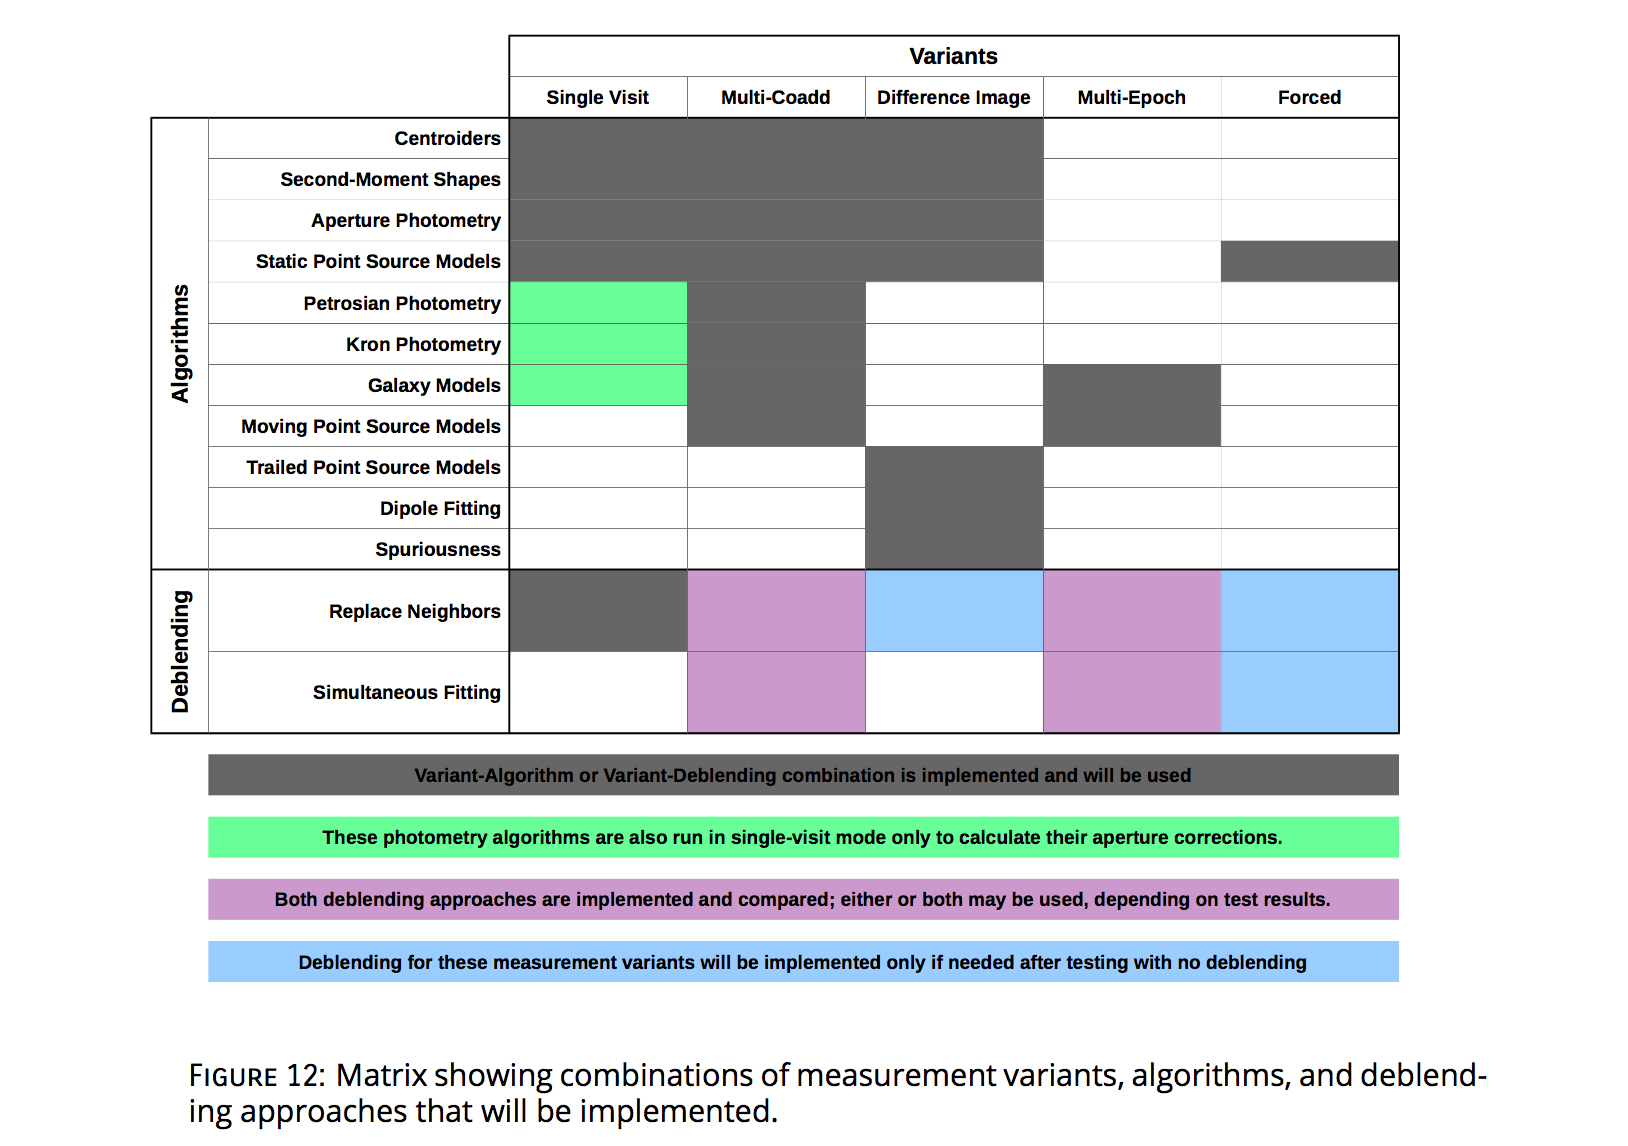
\includegraphics[width=\textwidth]{Figures/Figure12LDM-151.png}
    \label{fig:DM-fig12}
\end{figure}

Deblending is an integral part of the source detection and measurement pipeline, which makes isolating a ``deblending'' task challenging in itself. We want to allow several strategies, including neighbour masking/replacement and multi-object fitting.

\section{Dataset}

\begin{itemize}
\item Should we use simulated images or real images? Probably simulated images, because with real ones 1) you don't know the ground truth, and 2) its hard to stop competitors from matching them to external sources. 
\item What kind of simulator should we use to generate data? Is a simple parametric model good enough? Probably not, because with a simple parametric model, or even with a model based on a neural network, competitors who use the same kind of model for inference will have an advantage. That kind of advantage won't generalize to real data though, so it's not really what we want the competition to reward. With a complex, n-body type of simulation, it's pretty hard for a competitor to develop a technique that is better suited to the simulated data than the real data---even if the simulated data doesn't look perfectly realistic to the human eye.
\item Computationally intensive simulators are probably harder to ``game'' by methods that works well on simulated data but not real data. For that reason, we may want to consider simulators that run on GPUs. 
\item Should we distribute the simulator that generated the data, along with any setting we used, or to keep them secret? Probably we need to keep it secret. Because if competitors had access to the simulator, they could simulate images and train using the ground truth for them. That would work too well, effectively converting an unsupervised problem to a supervised one. We may also need to ban using external simulators to generate extra data.\\
\fl{Banning simulators is probably impossible to impose I think}\\
\jr{I agree that it would be nicer if we didn't have to ban anything, but maybe it's possible, for the following reasons:}\\
\jr{1. We would just need to ban n-body simulators, if that's how we generated the data, rather than all simulators. It's unlikely any contestant has a legitimate reason for using a n-body simulator as part of their solution.}\\
\jr{2. It's most difficult to enfoce a ban if there's a sizable prize at stake. If it's just a leaderboard for comparing algorithms, and no prize, we can probably count on participants to be follow the contest rules (``academic honesty'').}\\
\jr{3. Even for the Netflix prize (\$1 million prize) they banned using ``external'' information for predicting movie ratings, so a ban like this wouldn't be unprecedented. The winners had to submit their code to collect the prize so it was easily verified.}\\
\jr{4. If you can generate unlimited labeled data, you can just train a deep neural network to produce the right label for the data. You wouldn't even need to use the supplied training set, which wouldn't have labels, to train your algorithm. So somehow we have to keep users from generated their own labeled datasets---I think that means keeping the simulator secret or off limits}
\item What distribution should we draw the colors and fluxes for our simulated data from?
\item What PSF model should we use? Should we vary the PSF across the images, and give each image a timestamp? Or use a constant PSF?
\end{itemize}


\subsection{Known limitations}
We are not attempting to replicate every aspect of real data. Here are some known differences between our simulated data and real astronomical images.
\begin{itemize}
\item real galaxies are not transparent, especially within half-light radius
\item our images do not include gravitational lenses
\item our images do not show satellites, airplanes, planets, asteroids, etc.
\item we may have fewer, or less diverse, types of irregular galaxies in our simulated data
\end{itemize}


\section{Current deblenders}
We should add at least some of these to the leaderboard to serve as baselines.

\begin{itemize}
    \item SExtractor~\cite{bertin1996sextractor}
    \item HSC pipeline~\cite{bosch2018hyper}
    \item SCARLET~\cite{melchior2018scarlet}
\end{itemize}

\bibliography{references}{}
\bibliographystyle{unsrt}

\end{document}
